% !Mode:: "TeX:UTF-8"
%!TEX program = xelatex
% 问题二独立编译入口：在 Overleaf 中将 paper/ 目录作为项目根目录，
% 选择 XeLaTeX 编译本文件即可。
\documentclass[bwprint]{template/gmcmthesis}

\hypersetup{hidelinks}
\usepackage[framemethod=TikZ]{mdframed}
\usepackage{subfig}
\usepackage{siunitx}
\usepackage{colortbl}
\usepackage[noend]{algpseudocode}
\usepackage{algorithmicx,algorithm}
\usepackage{amsmath,amssymb,booktabs,graphicx}
\graphicspath{{./}{figures/q2-scaling-law/}{template/figures/}}
% 统一符号、命令和术语。新增命令先在这里登记。
\newcommand{\R}{\mathbb{R}}
\newcommand{\E}{\mathbb{E}}
\newcommand{\argmin}{\operatorname*{arg\,min}}


\title{问题二：跨维度数据融合与广义标度律}
\baominghao{待填写正式队伍编号}
\schoolname{学校名称填写}
\membera{成员 A}
\memberb{成员 B}
\memberc{成员 C}

\floatname{algorithm}{算法}
\renewcommand{\algorithmicrequire}{\textbf{输入:}}
\renewcommand{\algorithmicensure}{\textbf{输出:}}

\begin{document}
\maketitle

\begin{abstract}
本文针对参数规模、训练数据量、数据质量和领域配比来自不同附件、缺少逐行联合观测的问题，先分别检验规模项、质量增量和配比响应，再通过显式的质量桥接构造条件预测式。B1 内部留一检验支持幂律规模项；B6/B7 支持半合成质量增量的局部诊断；A 侧配方数据用于领域配比与质量代理的条件分析。结果显示，边际收益递减、有限领域替代和质量—参数替代均可在冻结模型内计算，但质量桥接覆盖有限，B8 存在方向冲突，B9/B10 仅支持范围审计，B4/B5 仍保留明显来源异质性。因此，本文将联合式定位为资源配置的条件情景模型，而非已经完成外部联合验证的广义定律。
\keywords{广义标度律\quad 数据质量\quad 领域配比\quad 条件外推\quad 迁移诊断}
\end{abstract}

\pagestyle{plain}
% 问题二候选正文；条件模型及 E1/E2 推导待独立科学评审。
% 正式论文由 paper/main.tex 集成；本文件可在审阅通过后直接 \input。
\section{跨维度数据融合与广义标度律}
\label{sec:q2}

\subsection{问题分析与数据口径}

题目要求将参数规模、训练数据量、数据质量和领域配比纳入统一的损失预测，并据此讨论资源的边际收益及领域之间的替代与互补。难点在于附件 A 与 B 并非同一批训练实验：A 侧包含领域配比和第一问得到的质量代理，B1 给出规模与训练量，B6/B7 给出质量扰动，但缺少同时观测四类输入及同一评价口径 Loss 的独立样本。因此先分别估计能够由数据支持的分项，再用显式的跨来源映射构造条件模型；分项验证和整个组合模型的有效性须分别判断。

记 $N$ 为十亿参数数，$D$ 为十亿训练 token 数，$L$ 为损失；$\boldsymbol p\in\Delta_{17}$ 为 17 个领域的训练占比，$\Delta_{17}=\{\boldsymbol p\geq\boldsymbol 0:\boldsymbol 1^\top\boldsymbol p=1\}$。第一问给出的领域质量分数组成 $\boldsymbol q$，定义 A 侧质量代理 $Q_A=\boldsymbol q^\top\boldsymbol p$。默认采用 TOPSIS 分数轴，同时以 soft 分数轴检查敏感性。这里 $Q_A$ 由配比确定，不能视作独立于 $\boldsymbol p$ 的一次质量干预。

表~\ref{tab:q2-data} 列出各数据块在本节的作用。所有 MAE 均按相应检验集的单行 Loss 计算；跨数据块的 MAE 因评价口径及基准 Loss 不同，不直接合并比较。

\begin{table}[htbp]
\centering
\caption{问题二使用的数据块与证据作用}
\label{tab:q2-data}
\begin{tabular}{p{0.15\linewidth}p{0.39\linewidth}p{0.37\linewidth}}
\toprule
数据块 & 已有观测及用途 & 证据边界 \\
\midrule
B1 & $N,D,L$；估计幂律规模项，8 个参数规模逐一留出 & 只验证 B1 文件内部规律 \\
B2、B4、B5 & 不同来源的 $N,D,L$；检验规模项迁移 & Loss 基准及训练轨迹有来源差异 \\
B6/B7、B8 & 带质量变量的实验；前两者估计及验证质量项，B8 隔离作方向诊断 & B6/B7 有重叠且属半合成数据；B8 分层方向未统一 \\
A4--A11 & 17 域配方及 A 侧平均 Loss；估计并检验配比响应 & 需目标规模校准，不能识别与 B1 绝对 Loss 的对齐 \\
B9/B10 & 大规模参数范围资料 & B9 为元数据，B10 Loss 为估算值，不构成真实外推检验 \\
\bottomrule
\end{tabular}
\end{table}

\subsection{分项估计与条件组合模型}

以题设幂律形式为规模基线，比较它与对数线性原型在相同 B1 留一规模划分上的外推误差。规模分项写为
\begin{equation}
L_{\mathrm{scale}}(N,D)=E+AN^{-\alpha}+BD^{-\beta},\qquad A,B,\alpha,\beta>0.
\label{eq:q2-scale}
\end{equation}
在 B1 上拟合得到 $E=1.689798$、$A=0.353980$、$B=1.240306$、$\alpha=0.339977$、$\beta=0.279878$。拟合支持范围为 $N\in[0.070542,11.965825]$、$D\in[0.134,299.893]$，单位均为十亿；两个区间各自的范围不意味着其任意笛卡尔积组合都有联合训练观测。

将 A 侧质量代理映射到 B7 质量坐标。仅用 A4/A5 的 512 个训练配方确定两条质量轴各自的 $q_{\min},q_{\max}$，令
\begin{equation}
T(Q_A)=\operatorname{clip}\!\left(0.1+0.9\frac{Q_A-q_{\min}}{q_{\max}-q_{\min}},\,0.1,\,1\right),
\qquad Q_{A0}=\boldsymbol q^\top\boldsymbol p_0,
\label{eq:q2-map}
\end{equation}
其中 $\boldsymbol p_0$ 为上述训练配方均值。此映射是把两套评分范围接合的假设，不是成对质量测量得到的经验标定。为避免将 $Q_A$ 和完整配比中同一方向重复计入，先在 A4/A5 训练集计算
\begin{equation}
\boldsymbol v=\frac{\sum_i(Q_{Ai}-Q_{A0})(\boldsymbol p_i-\boldsymbol p_0)}
{\sum_i(Q_{Ai}-Q_{A0})^2},\qquad
\boldsymbol r(\boldsymbol p)=\boldsymbol p-\boldsymbol p_0-\boldsymbol v(Q_A-Q_{A0}).
\label{eq:q2-residual}
\end{equation}
$\boldsymbol r$ 与 $Q_A$ 在训练样本上样本协方差为零，但这种线性残差化不等于统计独立，更不识别因果效应。令 $\widehat{\boldsymbol w}$ 为 A4/A5 上以 13 域平均 Loss 为目标、对 17 个中心化配比进行 Ridge 回归所得载荷，惩罚系数为 $10^{-5}$。质量斜率 $c=-0.361995$ 来自 B7；跨来源迁移强度 $\lambda_Q,\lambda_p\in\{0,0.5,1\}$ 为预设情景参数，而非联合数据估计值。冻结的组合式为
\begin{equation}
\boxed{\begin{aligned}
\widehat L_B(N,D,Q_A,\boldsymbol p)
={}&1.689798+0.353980N^{-0.339977}\\
&+1.240306D^{-0.279878}-0.361995\lambda_Q[T(Q_A)-T(Q_{A0})]\\
&+\lambda_p\widehat{\boldsymbol w}^{\top}\boldsymbol r(\boldsymbol p).
\end{aligned}}
\label{eq:q2-joint}
\end{equation}
式~\eqref{eq:q2-joint} 的输出以 B1 Loss 为参照。B7 的来源截距没有加到该式，A 侧平均 Loss 的绝对水平也没有直接移入；因此它是用于比较方案的\textbf{条件预测式}，不是已经由共同观测样本识别和验收的广义定律。

\subsection{分层检验与迁移结果}

留一规模检验在 B1 的 8 折共汇总 1176 行。幂律的 MAE/RMSE 为 $0.000108/0.000151$，对数线性原型为 $0.090739/0.123077$，故选式~\eqref{eq:q2-scale} 为该文件的规模项。图~\ref{fig:q2-b1} 逐折给出留出误差；点之间不连线，因为规模折彼此独立。B1 的近乎精确拟合反映该附件与幂律形式高度一致，不可解释为真实训练损失没有噪声。锁定 B1 参数直接预测 B2、B4、B5，MAE 分别升至 $1.178442$、$0.227263$、$0.170722$，显示绝对 Loss 存在来源差异。

\begin{figure}[htbp]
\centering
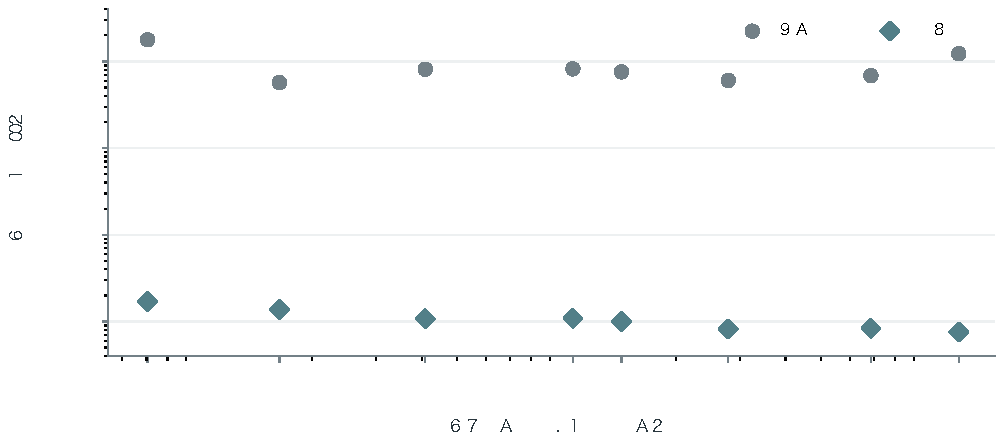
\includegraphics[width=0.88\linewidth]{figures/q2-scaling-law/Fig01_B1_leave_size.pdf}
\caption{B1 留一参数规模验证。8 折各留出一个规模、每折 147 行；散点为每折 MAE，横纵轴均取对数。此图反映 B1 内部表现。}
\label{fig:q2-b1}
\end{figure}

质量项验证冻结 B1 规模参数，并让“无 $Q$”基线与“加 $Q$”模型使用相同的来源截距。B7 按 $(N,D)$ 组合分组留出时，MAE 从 $0.101965$ 降至 $0.057322$；留出完整质量水平时，从 $0.110407$ 降至 $0.057046$；用 B6 训练并仅预测 B7 中不重叠的新增 90 行时，从 $0.057491$ 降至 $0.044603$（图~\ref{fig:q2-quality}）。这些比较支持半合成机制内的质量增量，却不提供真实语料质量提高后的独立训练效果；分组结果还参与线性质量形式的选择，不能充作最终盲测。

\begin{figure}[htbp]
\centering
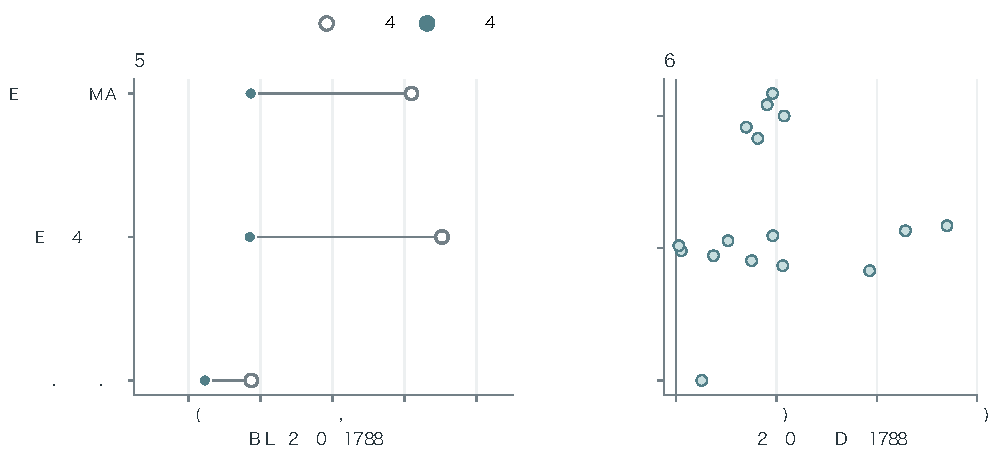
\includegraphics[width=0.9\linewidth]{figures/q2-scaling-law/Fig02_quality_increment.pdf}
\caption{引入 $Q$ 后的误差变化。a 为相同来源截距下的汇总 MAE；b 为各留出折的 MAE 改善量。B6 到 B7 的检验只计不重叠的新增 90 行，B6/B7 属半合成数据。}
\label{fig:q2-quality}
\end{figure}

对跨来源偏移另作嵌套留出：外层留出 B2 的完整训练轨迹，内层选择校准形式；A 侧按不同配方进行外层留出与内层选择。表~\ref{tab:q2-transfer} 记录外层汇总值，图~\ref{fig:q2-transfer} 显示逐折误差。B2 校准后虽优于均值基线，残差与 $\log D$ 的 Spearman 相关仍约为 $0.9961$--$0.9979$，表明截距校正没有消除曲线形状偏差。A 60M 可经目标规模标签校准改善；A 1B 的选择模型未超过均值，故没有统一的跨规模配比迁移系数。

\begin{table}[htbp]
\centering
\caption{来源与配比迁移的外层留出 MAE（数值越低越好）}
\label{tab:q2-transfer}
\begin{tabular}{lrrr}
\toprule
目标来源 & 未校准 & 嵌套选择 & 简单均值基线 \\
\midrule
B2 规模轨迹（1029 行） & 1.178442 & 0.266023 & 0.372331 \\
A 60M 配方（256 行） & 1.508086 & 0.146142 & 0.167310 \\
A 1B 配方（64 行） & 3.190256 & 0.040878 & 0.039563 \\
\bottomrule
\end{tabular}
\end{table}

\begin{figure}[htbp]
\centering
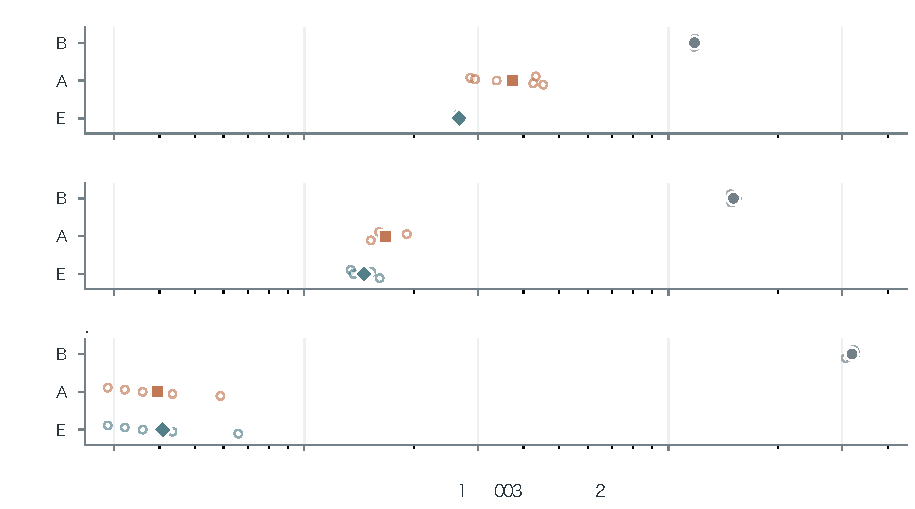
\includegraphics[width=0.9\linewidth]{figures/q2-scaling-law/Fig03_transfer_calibration.pdf}
\caption{迁移到 B2、A 60M 和 A 1B 时的外层误差。实心点为所有外层行汇总的 MAE，空心点为单折 MAE；校准形式仅由内层训练数据选择。A 1B 选择模型的汇总误差高于均值基线。}
\label{fig:q2-transfer}
\end{figure}

A6/A7 的 256 行同规模配比检验中，完整配比模型的 MAE 为 $0.180679$，训练均值基线为 $0.225599$。质量残差配比模型为 $0.184309$；把 A 侧质量分量替换为 B7 质量斜率并保留 A 训练截距后为 $0.180795$。这只支持 A 侧的局部组件替换。跨规模时，扣除各测试集均值的配比形状 RMSE 在 60M 为 $0.1943$，低于常数模型的 $0.2189$；到 1B 时为 $0.1615$，高于常数模型的 $0.0519$（图~\ref{fig:q2-mixture}）。该中心化指标使用测试集均值，不能当作无需目标标签的部署误差。

\begin{figure}[htbp]
\centering
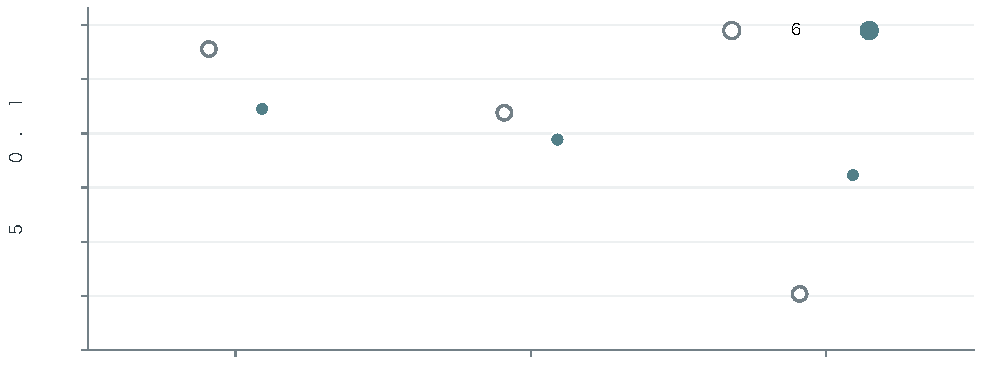
\includegraphics[width=0.86\linewidth]{figures/q2-scaling-law/Fig04_mixture_scale.pdf}
\caption{A 侧不同参数规模的配比响应形状。完整配比模型与均值基线按规模并列；纵轴为中心化 RMSE，仅检验配比响应形状。1B 结果不支持固定迁移 1M 的配比幅度。}
\label{fig:q2-mixture}
\end{figure}


\subsection{边际收益、弹性与等效规模条件}

将式~\eqref{eq:q2-joint} 的质量和配比固定，定义单位资源带来的正向 Loss 改善率 $U_N=-\partial\widehat L_B/\partial N$、$U_D=-\partial\widehat L_B/\partial D$。于是
\begin{equation}
\begin{aligned}
U_N&=\alpha AN^{-\alpha-1}, & U_D&=\beta BD^{-\beta-1},\\
\frac{\partial^2\widehat L_B}{\partial N^2}&=\alpha(\alpha+1)AN^{-\alpha-2}>0,\\
\frac{\partial^2\widehat L_B}{\partial D^2}&=\beta(\beta+1)BD^{-\beta-2}>0.
\end{aligned}
\label{eq:q2-marginal}
\end{equation}
正的二阶导数表示增加资源后损失下降的幅度递减。对\emph{完整} Loss 的弹性为
\begin{equation}
\varepsilon_N=-\frac{\alpha AN^{-\alpha}}{\widehat L_B},\qquad
\varepsilon_D=-\frac{\beta BD^{-\beta}}{\widehat L_B}.
\label{eq:q2-elasticity}
\end{equation}
在 $N=1$、$D=100$、$\boldsymbol p=\boldsymbol p_0$ 和 $\lambda_Q=\lambda_p=1$ 的计算锚点，$\widehat L_B=2.385578$，$U_N=0.120345$、$U_D=0.000957$，$\varepsilon_N=-0.050447$、$\varepsilon_D=-0.040100$。$U_N$ 和 $U_D$ 的单位分别是每十亿参数和每十亿 token 的局部 Loss 变化，不能凭数值大小比较资金效率；两种资源翻倍后，各自的单位边际收益变为原来的 $39.50\%$ 和 $41.18\%$。本锚点是模型计算，未对应新增的四变量联合观测。

在质量映射的内部区间，若沿保持 $\boldsymbol r$ 不变的条件路径改变 $Q_A$，则
\begin{equation}
\left.\frac{\partial\widehat L_B}{\partial Q_A}\right|_{\boldsymbol r}
=c\lambda_Q\frac{0.9}{q_{\max}-q_{\min}},\qquad c=-0.361995;
\label{eq:q2-quality-derivative}
\end{equation}
截断区该形式导数为零，边界处只定义单侧导数。TOPSIS 和 soft 轴在 $\lambda_Q=1$ 时的内区斜率分别为 $-2.605474$ 和 $-0.675302$，两轴的分数单位不同，斜率绝对值不能直接比较。质量弹性还依赖分数原点，故仅在同一评分定义下解释。

题目所问的“质量提高 $0.1$ 等效增加多少参数”必须先指定质量单位。设映射后的 B 侧质量坐标 $z=T(Q_A)$ 增加 $\Delta z=0.1$，且变化全程处于线性区、$D$ 及剩余配比分量保持不变。令增加参数后的规模收益等于质量收益，则
\begin{equation}
A\{N_{\mathrm{eq}}^{-\alpha}-N^{-\alpha}\}=c\lambda_Q\Delta z,
\qquad
N_{\mathrm{eq}}=\left(N^{-\alpha}+\frac{c\lambda_Q\Delta z}{A}\right)^{-1/\alpha},
\label{eq:q2-equivalent}
\end{equation}
前提为括号内严格为正，且 $N_{\mathrm{eq}}$ 位于经验支持范围。以 $N=1$、$\lambda_Q=1$ 代入，得到 $N_{\mathrm{eq}}\approx1.373$，即模型中映射质量轴增加 $0.1$ 的 Loss 改善，约等于参数从 10 亿增至 13.73 亿。若题目中的 $0.1$ 指 A 侧原始代理 $Q_A$，应以 $\Delta z=T(Q_A+0.1)-T(Q_A)$ 代入，数值依赖起点和截断，不能直接沿用 13.73 亿。由于 A 侧 $Q_A=\boldsymbol q^\top\boldsymbol p$，保持剩余配比不变是计算路径，不是独立质量实验。若进一步比较资金投入，还需给出参数扩容与质量提升的成本函数；现有附件不能确定货币意义下的最优选择。

\begin{figure}[htbp]
\centering
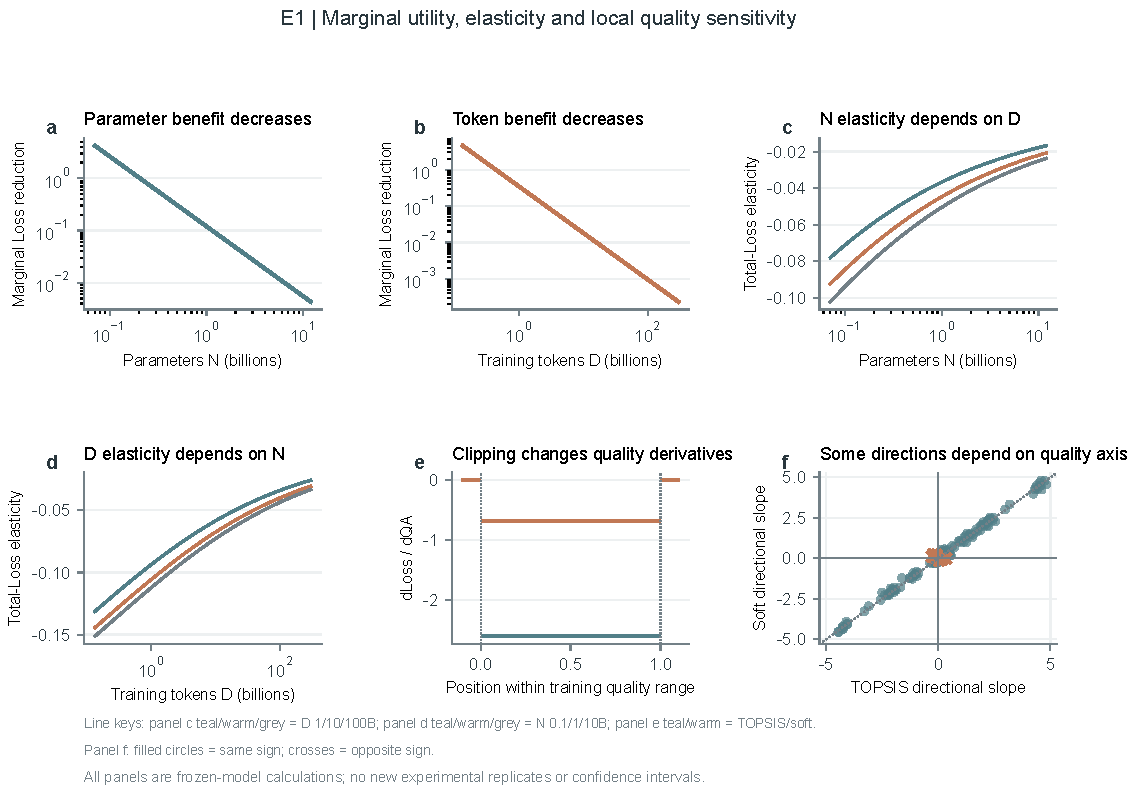
\includegraphics[width=0.96\linewidth]{figures/q2-scaling-law/Fig05_E1_marginal_elasticity.pdf}
\caption{冻结模型下的边际效用、弹性和局部质量敏感性。a,b 展示参数与训练 token 的边际 Loss 改善递减；c,d 展示弹性随另一项规模变量变化；e 展示质量映射在截断区与内部区的导数；f 比较两条质量轴对领域方向导数的符号。所有面板均为条件计算，不含新的联合训练观测。}
\label{fig:q2-e1}
\end{figure}

\subsection{领域替代、互补与情景敏感性}

固定总训练量，令 $\boldsymbol p(\delta)=\boldsymbol p_0+\delta(\boldsymbol e_i-\boldsymbol e_j)$ 表示从领域 $j$ 向 $i$ 转移配比 $\delta$。在质量映射内部，冻结模型给出
\begin{equation}
\boldsymbol g=\nabla_{\boldsymbol p}\widehat L_B
=c\lambda_Q\frac{0.9}{q_{\max}-q_{\min}}\boldsymbol q
+\lambda_p\{\widehat{\boldsymbol w}-(\widehat{\boldsymbol w}^{\top}\boldsymbol v)\boldsymbol q\},
\qquad \frac{\mathrm d\widehat L_B}{\mathrm d\delta}=g_i-g_j.
\label{eq:q2-substitution}
\end{equation}
$\delta=0.01$ 表示 1 个百分点；$g_i-g_j<0$ 表示模型预测转移后 Loss 降低。为限制推论范围，对 272 个有向领域对求解训练配方凸包内的最大转移量，并以最优边界的 $99\%$ 作安全上限。0.1、0.5、1、2、5 个百分点分别有 272、256、224、165、117 个方向通过该上限；安全上限的中位数为 4.068 个百分点。特征支持只表示可由已有训练配方凸组合构造，不表示该方向已做真实训练验证。

在 $\lambda_Q=\lambda_p=1$ 时，136 个无序领域对中有 12 对在 TOPSIS 与 soft 质量轴下预测方向相反。扩大到 $\lambda_Q,\lambda_p\in\{0,0.5,1\}$ 的非全零情景后，107 对出现正负翻转；这包含关闭某一分项的压力情景，不是翻转概率。因而不依据式~\eqref{eq:q2-substitution} 排列全局领域优劣。

为检查模型能否刻画互补，取共同供给领域 $k$，使 $\boldsymbol p_{10}=\boldsymbol p_0+h(\boldsymbol e_i-\boldsymbol e_k)$、$\boldsymbol p_{01}=\boldsymbol p_0+h(\boldsymbol e_j-\boldsymbol e_k)$，并令 $\boldsymbol p_{11}=\boldsymbol p_0+h(\boldsymbol e_i+\boldsymbol e_j-2\boldsymbol e_k)$。定义四角差
\begin{equation}
I_{ij\mid k}=\widehat L_B(\boldsymbol p_{11})-\widehat L_B(\boldsymbol p_{10})
-\widehat L_B(\boldsymbol p_{01})+\widehat L_B(\boldsymbol p_0).
\label{eq:q2-interaction}
\end{equation}
在 A4 配方凸包内的 2040 个四角设计、两条质量轴共 4080 次条件计算中，$\max|I_{ij\mid k}|=8.88\times10^{-16}$ Loss，处于数值零水平。原因是映射内部式~\eqref{eq:q2-joint} 关于 $\boldsymbol p$ 为仿射函数；零交互是模型结构强制的，不能证明真实领域之间没有互补。凸包外质量映射截断可产生非零四角差，同样不能解释为真实互补。

由于式~\eqref{eq:q2-joint} 中 $N,D$ 与质量、配比项可加分离，固定配比下 $U_N,U_D$ 不随质量情景改变；质量与配比影响式~\eqref{eq:q2-elasticity} 的分母，并影响领域转移方向。它不能在没有成本耦合的前提下证明质量会改变最优 $N/D$。若将来取得相同 $N,D$、统一评价集下不同质量与四角配方的真实重复训练，可再估计跨块交互和实际互补强度。

\begin{figure}[htbp]
\centering
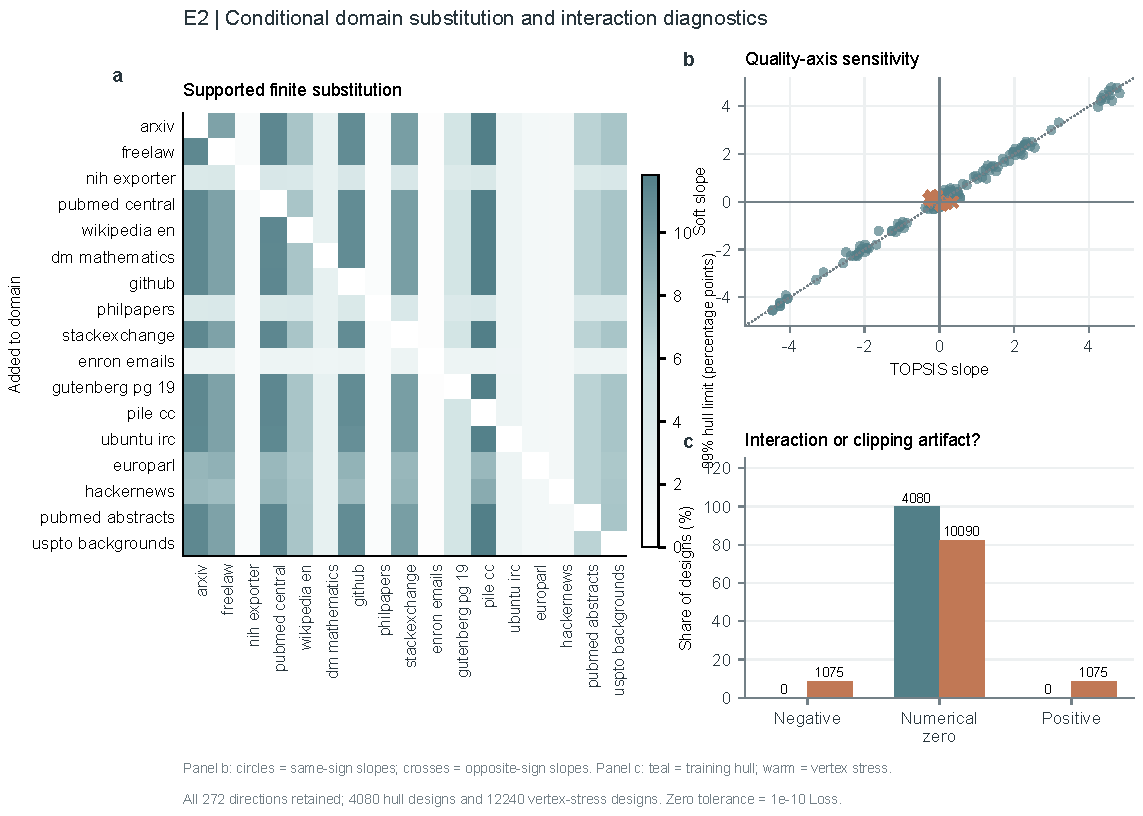
\includegraphics[width=0.96\linewidth]{figures/q2-scaling-law/Fig06_E2_substitution_interaction.pdf}
\caption{有条件的领域替代与交互诊断。a 为 17 个领域之间的安全替代幅度；b 为两条质量轴下领域方向斜率的一致性；c 比较训练配方凸包和凸包外顶点压力情景中的四角差符号。热图表示已有配方支持的有限替代范围，不表示真实训练干预已经完成。}
\label{fig:q2-e2}
\end{figure}

\subsection{质量—参数替代的可行性边界}

质量分数提高并不自动对应可实现的配方变化。我们沿固定剩余配比效应的路径 $\boldsymbol p(t)=\boldsymbol p_0+t\boldsymbol v$，并把质量收益换算为保持原预测 Loss 所需的参数规模。设 $G$ 为固定规模下的预测 Loss 改善，$S=A N_0^{-\alpha}$ 为原参数项，则保持原 Loss 的等效参数规模为
\begin{equation}
N_{\mathrm{required}}=\left(\frac{S+G}{A}\right)^{-1/\alpha},
\label{eq:q2-required-scale}
\end{equation}
其中要求 $S+G>0$，且质量路径端点位于训练配方凸包支持内。若只使用形式质量坐标而不限制配方可行性，得到的等效扩张会显著偏大。

在 $N_0=1$、$D=100$、$\lambda_Q=\lambda_p=1$ 的条件下，TOPSIS 质量轴的 99\% 可行路径端点对应约 $1.393$ 倍的形式规模，soft 质量轴约为 $1.940$ 倍；若忽略配方可行性，两个数值分别上升到约 $2.389$ 和 $9.218$ 倍（图~\ref{fig:q2-e3}）。同一计算还发现，512 个训练配方中分别有 144 个 TOPSIS 情景和 70 个 soft 情景出现“质量上升但总预测 Loss 未改善”的反例。因此，质量代理只能在明确路径和约束下解释，不能单独推出缩参结论。

\begin{figure}[htbp]
\centering
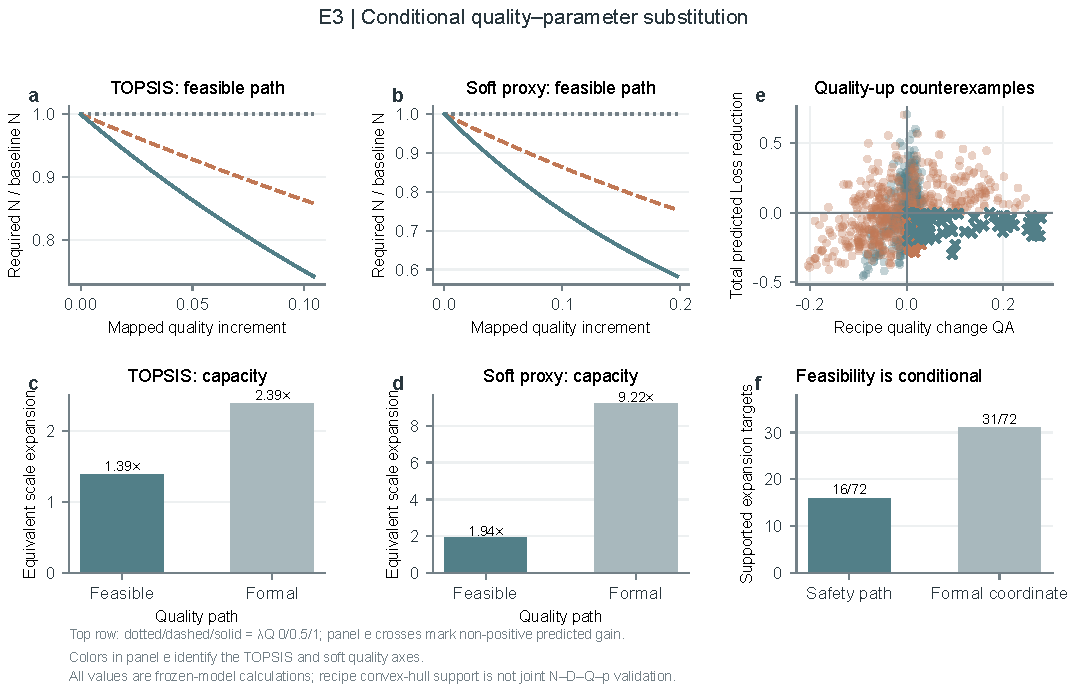
\includegraphics[width=0.96\linewidth]{figures/q2-scaling-law/Fig07_E3_quality_parameter_tradeoff.pdf}
\caption{质量—参数替代的可行性边界。a,b 给出 TOPSIS 与 soft 质量轴下的可行路径；c,d 比较可行路径与形式质量坐标的等效规模扩张；e 展示质量上升但总预测收益非正的配方反例；f 汇总可支持的扩张目标数。}
\label{fig:q2-e3}
\end{figure}

\subsection{质量桥接、范围外推与来源异质性}

A 与 B 的质量变量分别基于各自数据进行构造与分析，二者对应不同的样本观测关系。17 个领域中有 3 个可以直接对应，另有 3 个属于近似语义对应，剩余 11 个需要推断映射；在配方质量代理中，1M 和 60M 验证配方的平均可映射质量占比分别约为 $0.569$，1B 配方约为 $0.622$，其余质量信息仍未被覆盖。图~\ref{fig:q2-bridge} 将这一覆盖缺口与 A--B 接口的可识别性边界并列展示。这里的“可映射质量占比”是特征覆盖诊断，不是经过共同样本校准的质量测量。

\begin{figure}[htbp]
\centering
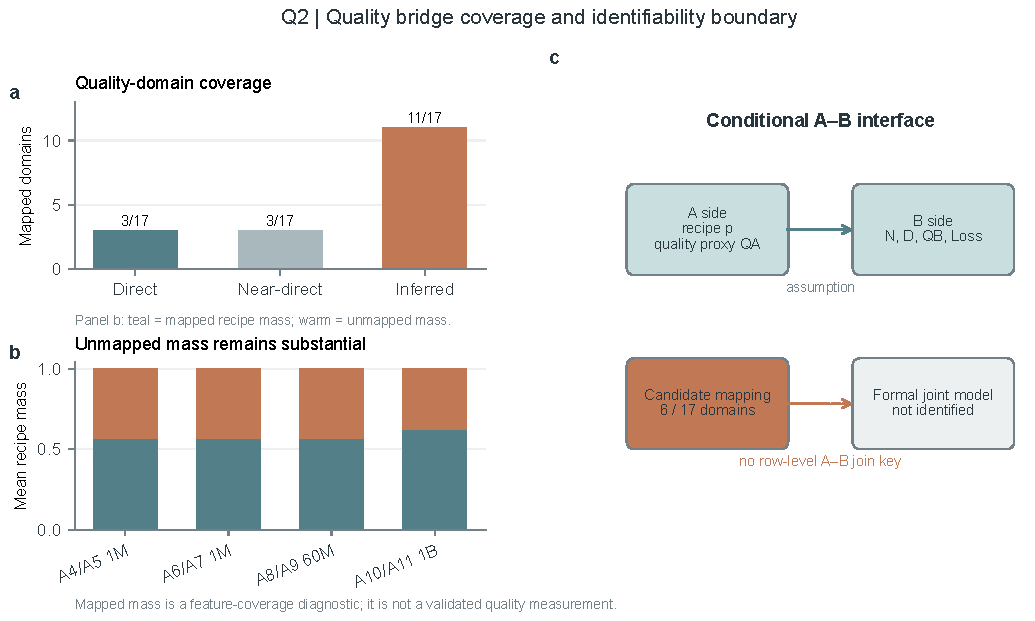
\includegraphics[width=0.96\linewidth]{figures/q2-scaling-law/Fig09_quality_bridge_coverage.pdf}
\caption{A--B 质量桥接覆盖与可识别性边界}
\label{fig:q2-bridge}
\end{figure}

B9 提供参数和训练量范围，B10 的 Loss 为估算值，二者不能用作外部预测精度验证。相对于 B1 的参数支持区间 $[0.070542,11.965825]$ 十亿，B9/B10 的最大参数规模为 10,000B，约为 B1 上界的 $835.7$ 倍；训练量上界为 36,000B，约为 B1 上界的 $120.0$ 倍。图~\ref{fig:q2-e4} 因此报告范围条件下的情景轨迹，并明确标出 B1 支持范围。

\begin{figure}[htbp]
\centering
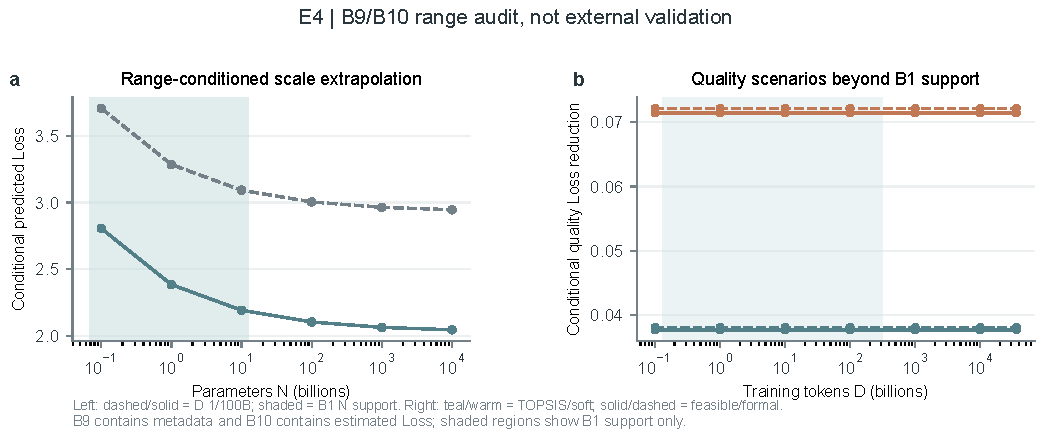
\includegraphics[width=0.96\linewidth]{figures/q2-scaling-law/Fig08_E4_scale_extrapolation.pdf}
\caption{B9/B10 范围审计}
\label{fig:q2-e4}
\end{figure}

最后，我们按照模型家族和文献来源对 B4/B5 的外部诊断结果进行分层汇报，并分别依据各来源的评价口径解释相应误差指标。B4 各家族的 MAE 从约 $0.057$ 到 $0.443$ 不等，Pythia 的误差最高；B5 各文献来源的 MAE 从约 $0.123$ 到 $0.308$ 不等，Chowdhery 等来源的组内误差最高。小组样本量为 1--4 的组仅作诊断，并未重新拟合模型；分层差异说明跨来源误差异质性仍然存在（图~\ref{fig:q2-stratified}）。

\begin{figure}[htbp]
\centering
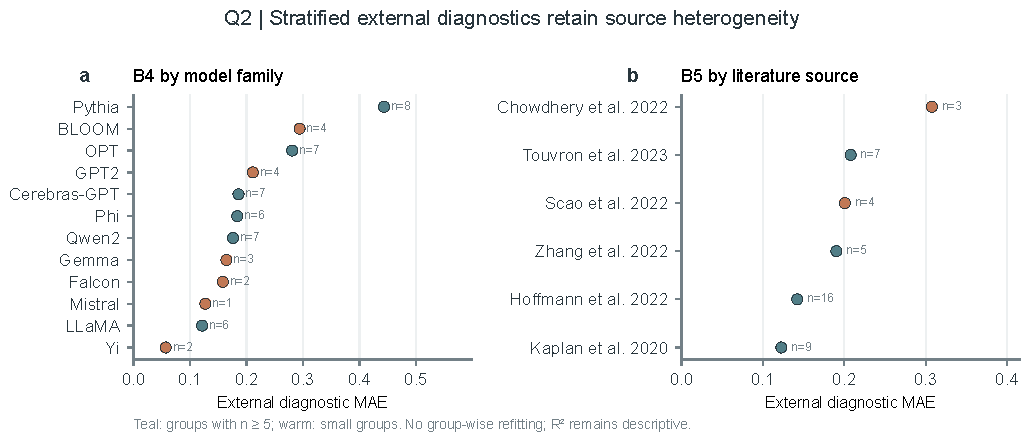
\includegraphics[width=0.96\linewidth]{figures/q2-scaling-law/Fig11_stratified_transfer_diagnostics.pdf}
\caption{B4/B5 外部诊断的分层结果}
\label{fig:q2-stratified}
\end{figure}

\subsection{适用范围与待验证结论}

图~\ref{fig:q2-b8} 显示 B8 的组内质量方向与 B6/B7 不完全一致，因此 B8 未参与质量斜率估计。图~\ref{fig:q2-range} 将 B1 拟合支持范围与 B9/B10 的参数范围并列；参数规模延伸只给出外推情景，不等于预测精度验证。

B8 的 1,704 个质量步中，1,311 个对应 Loss 上升，2 个下降，另有 241 个数值上为零；其中 984 行属于校准或继承范围，720 行属于外推范围（图~\ref{fig:q2-b8-new}）。这与 B6/B7 的方向分布不同，不能在缺少生成记录的情况下静默翻转或合并。因此，B8 被保留为数据语义和方向一致性的诊断，而不是质量斜率的训练样本。

\begin{figure}[htbp]
\centering
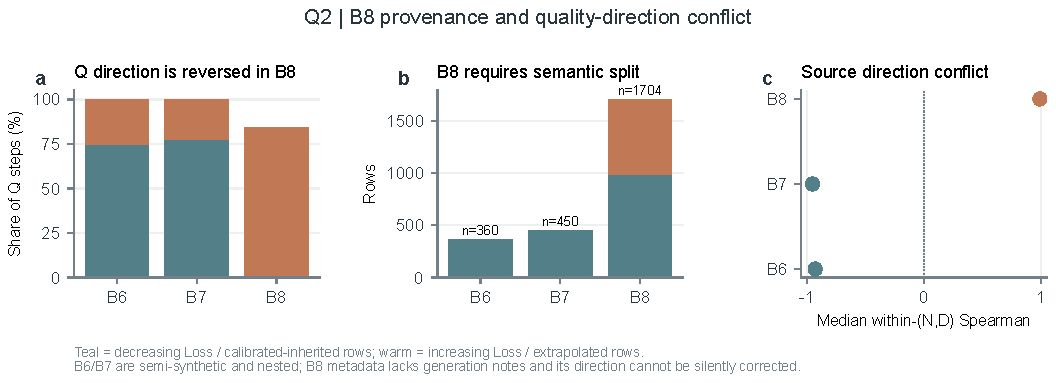
\includegraphics[width=0.96\linewidth]{figures/q2-scaling-law/Fig10_B8_direction_conflict.pdf}
\caption{B8 的质量方向冲突与来源拆分。a 比较 B6、B7、B8 的质量步方向；b 拆分校准/继承与外推行；c 给出固定 $(N,D)$ 组内的中位 Spearman 方向。B8 的异常方向只用于诊断，不作为静默修正依据。}
\label{fig:q2-b8-new}
\end{figure}

\begin{figure}[htbp]
\centering
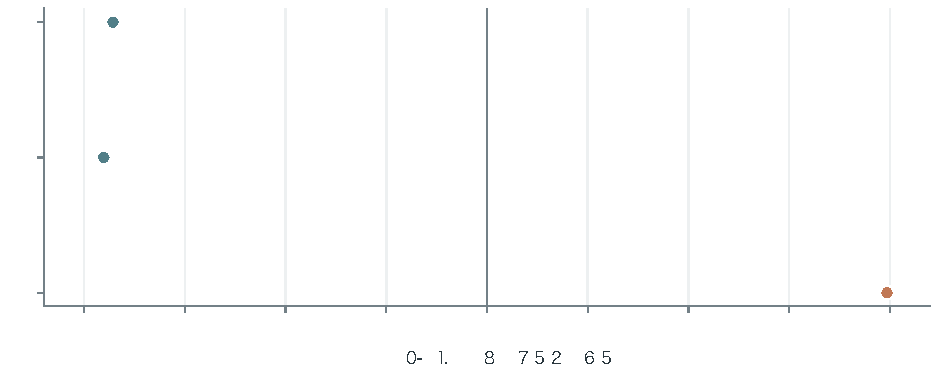
\includegraphics[width=0.82\linewidth]{figures/q2-scaling-law/FigS01_B8_quality_direction.pdf}
\caption{B6、B7、B8 在固定 $(N,D)$ 组内的质量--Loss Spearman 相关中位数。B7 包含 B6，二者不能作为独立重复实验；B8 留作方向诊断。}
\label{fig:q2-b8}
\end{figure}

\begin{figure}[htbp]
\centering
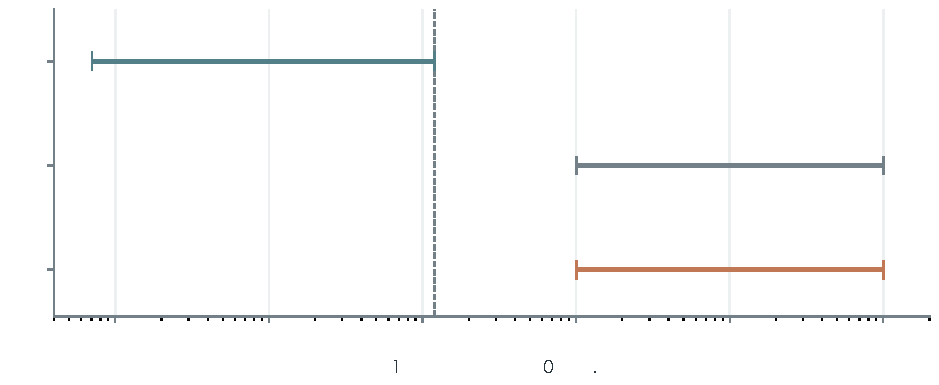
\includegraphics[width=0.82\linewidth]{figures/q2-scaling-law/FigS02_large_model_range.pdf}
\caption{B1 主拟合、B9 元数据与 B10 估算材料的参数范围。虚线为 B1 的最大参数规模；B9 缺少此图可用的实测 Loss，B10 Loss 为估算值。}
\label{fig:q2-range}
\end{figure}

现阶段可以回答：B1 内部幂律优于对数线性原型；半合成 B6/B7 中质量项有局部增量；A 侧同规模配比有预测信息；条件模型的边际效用递减、可行替代范围和结构性零交互可由公式及数值核查。尚不能给出整个 $N,D,Q_A,\boldsymbol p$ 模型的独立联合误差、真实质量干预收益、领域互补强度或无条件的大模型外推准确率。后续须获取共同观测四类输入及同口径 Loss 的训练实验，并在模型与质量映射冻结后留出独立测试集；在此之前，式~\eqref{eq:q2-joint} 只能作为资源配置情景分析的条件目标函数。


\end{document}
